\section{An integrated matrix trace inequality}\label{sec:trace}

The matrix step in the proof compares an integrated resolvent
difference with the Hermitian perturbation that produces it.
We prove the comparison for matrices of arbitrary size.  The
perturbation may be indefinite; positivity is imposed on the entire
symbol.

For the fixed exponent $0<\sigma<1$, define $c_\sigma>0$ by
\begin{equation}\label{eq:trace-normalization}
 c_\sigma^{-1}
 =\int_0^\infty t^\beta
       \bigl(t^{-1/2}-(t+1)^{-1/2}\bigr)\,dt.
\end{equation}
Recall that $\beta=\sigma-\tfrac12\in(-\tfrac12,\tfrac12)$.
The integrand in \eqref{eq:trace-normalization} is
$O(t^{\beta-1/2})$ at zero and $O(t^{\beta-3/2})$ at infinity.
The integral is therefore finite, and scaling gives
\begin{equation}\label{eq:trace-scaling}
 c_\sigma\int_0^\infty t^\beta
       \bigl(t^{-1/2}-(t+y)^{-1/2}\bigr)\,dt=y^\sigma,
 \qquad y\geq0.
\end{equation}

\begin{theorem}[Integrated trace comparison]\label{thm:trace}
Let $n\geq1$ and let $B,V\in\C^{n\times n}$ be Hermitian.
Suppose that for some $b>0$,
\begin{equation}\label{eq:trace-symbol}
 Y_s=(sI-B)^2,\qquad X_s=Y_s+V\geq bI
 \qquad\text{for every }s\in\R.
\end{equation}
For $t>0$, set
\begin{equation}\label{eq:trace-resolvents}
 R(t)=\frac1\pi\int_\R(X_s+tI)^{-1}\,ds,
 \qquad P(t)=t^{-1/2}I-R(t),
\end{equation}
and define
\begin{equation}\label{eq:trace-N}
 N=c_\sigma\int_0^\infty t^\beta P(t)\,dt.
\end{equation}
These integrals converge absolutely in matrix norm.  If $N\geq0$, then
\begin{equation}\label{eq:trace-comparison}
                         \tr(NV)\geq\tr(N^q).
\end{equation}
\end{theorem}

For a scalar $V=v>0$, shifting the variable $s$ gives
$R(t)=(t+v)^{-1/2}$ and $N=v^\sigma$.  Thus the two sides of
\eqref{eq:trace-comparison} agree in the scalar case.  To retain this
constant for noncommuting matrices, we will express the difference in
\eqref{eq:trace-comparison} as an integral of nonnegative terms.
The first step computes the resolvent through solutions of a
constant-coefficient equation on the two half-lines.

\subsection{Resolvent estimates and half-line solutions}

We first verify convergence.  The matrices $X_s$ and $Y_s$ grow
quadratically as $|s|\to\infty$.  Combined with the lower bound in
\eqref{eq:trace-symbol}, this shows that $X_s^{-1}$ has an integrable
matrix-norm bound on $\R$.  Consequently $R(t)>0$ and $R(t)=O(1)$ as
$t\downarrow0$.  Diagonalizing $B$ gives
\[
 \frac1\pi\int_\R(Y_s+tI)^{-1}\,ds=t^{-1/2}I.
\]
For $t\geq1$, both $X_s+tI$ and $Y_s+tI$ are bounded below by
$c(s^2+t)I$ for some $c>0$ independent of $s,t$.  The resolvent
identity, with the fixed matrix difference $V$, therefore gives
\begin{equation}\label{eq:trace-P-bounds}
 \|P(t)\|=
 \begin{cases}
  O(t^{-1/2}),&t\downarrow0,\\
  O(t^{-3/2}),&t\to\infty.
 \end{cases}
\end{equation}
For the second estimate, the norm of the difference of the two
resolvents is at most $C(s^2+t)^{-2}$, whose $s$-integral is
$O(t^{-3/2})$.  The range of $\beta$ now proves the absolute
convergence in \eqref{eq:trace-N}.

Matrix Riccati equations also underlie the commutation approach to
matrix Schr\"odinger inequalities \cite{BenguriaLoss2000}.  Here the
boundary matrices will compute both a resolvent integral and a
logarithmic determinant integral.  Fix $t>0$, write
$\nabla=\partial_x-iB$, and consider
\begin{equation}\label{eq:trace-ode}
                    (-\nabla^2+V+tI)\psi=0.
\end{equation}
The following construction relates its decaying solutions to $R(t)$.

\begin{lemma}\label{lem:trace-half-lines}
For every $v\in\C^n$, equation \eqref{eq:trace-ode} has a unique
$H^1$ solution on each half-line with boundary value $v$ at zero.
There are Hermitian matrices $S=S(t)$ and $T=T(t)$ such that these
solutions satisfy
\begin{equation}\label{eq:trace-boundary-maps}
 \nabla\psi(0+)=-Sv,\qquad \nabla\psi(0-)=Tv,
\end{equation}
respectively.  They obey
\begin{equation}\label{eq:trace-riccati}
 V+tI=S^2+i[B,S]=T^2-i[B,T],
 \qquad \frac{S+T}{2}=R(t)^{-1}.
\end{equation}
Every eigenvalue of $B+iS$ has strictly positive imaginary part.
\end{lemma}

\begin{proof}
With inner products linear in the second argument, let
\[
 a_t(\phi,\psi)=\int
    \bigl(\langle\nabla\phi,\nabla\psi\rangle
       +\langle\phi,(V+tI)\psi\rangle\bigr)\,dx.
\]
On the full line its Fourier symbol is $X_s+tI$, and
\eqref{eq:trace-symbol} and quadratic growth give
$X_s+tI\geq c_t(1+s^2)I$ for some $c_t>0$.
Thus $a_t$ is coercive on $H^1(\R;\C^n)$.  Zero extension proves
the same assertion on the subspace of $H^1$ functions on either
half-line whose boundary trace is zero.

Choose any $H^1$ extension $\eta$ of the prescribed boundary value.
On the trace-zero space the form $a_t$ is an equivalent Hilbert
space inner product.  The Riesz representation theorem gives a
unique correction $u$ in that space with
$a_t(\phi,u)=-a_t(\phi,\eta)$ for every trace-zero $\phi$.
Then $\psi=\eta+u$ solves \eqref{eq:trace-ode} weakly.
Conversely, an $H^1$ solution satisfies this weak identity by
density of interior test functions in the trace-zero space, so
coercivity proves uniqueness.

The equation implies $\psi''\in L^2$.  In particular the solutions
belong to $H^2$, their first derivatives have boundary traces, and
both $\psi$ and $\psi'$ tend to zero at the infinite end of the
half-line.  Define $S$ and $T$ by \eqref{eq:trace-boundary-maps}.
For the right solutions with data $v,w$, integration by parts gives
$a_t(\psi_v,\psi_w)=\langle v,Sw\rangle$; on the left it gives
$a_t(\psi_v,\psi_w)=\langle v,Tw\rangle$.  Since $a_t$ is Hermitian,
both boundary matrices are Hermitian.

Translation and uniqueness imply the same derivative relations
at every interior point:
\[
 \nabla\psi=-S\psi\quad\text{on }(0,\infty),\qquad
 \nabla\psi=T\psi\quad\text{on }(-\infty,0).
\]
For example,
$\nabla(-S\psi)=-S\nabla\psi+i[B,S]\psi$.
Substitution into \eqref{eq:trace-ode}, followed by evaluation at
zero for arbitrary boundary data, proves the two Riccati identities
in \eqref{eq:trace-riccati}.

Glue the right and left solutions with the same value $v$ at zero.
Figure~\ref{fig:half-line-gluing} records the boundary signs and
the normalization in this gluing identity.
The resulting function is continuous, and its derivative has jump
$-(S+T)v$.  On the full line it therefore satisfies
\[
 (-\nabla^2+V+tI)\psi=\delta_0(S+T)v.
\]
Using the Fourier transform with forward kernel $e^{-isx}$ and
inverting at zero gives
\[
 v=\frac1{2\pi}\int_\R(X_s+tI)^{-1}\,ds\,(S+T)v
   =\frac12R(t)(S+T)v.
\]
This inversion may first be taken in tempered distributions;
the transformed function is integrable because the inverse symbol
is $O(s^{-2})$, so evaluation at zero is legitimate.  Since
$R(t)>0$, the second identity in \eqref{eq:trace-riccati} follows.

Finally the right solutions satisfy $\psi'=i(B+iS)\psi$.
If $(B+iS)v=zv$ with $v\ne0$, uniqueness for this first-order
initial-value problem gives $\psi(x)=e^{izx}v$.
It belongs to $L^2(0,\infty;\C^n)$, hence
$\operatorname{Im}z>0$.
\end{proof}

\begin{figure}[tb]
 \centering
 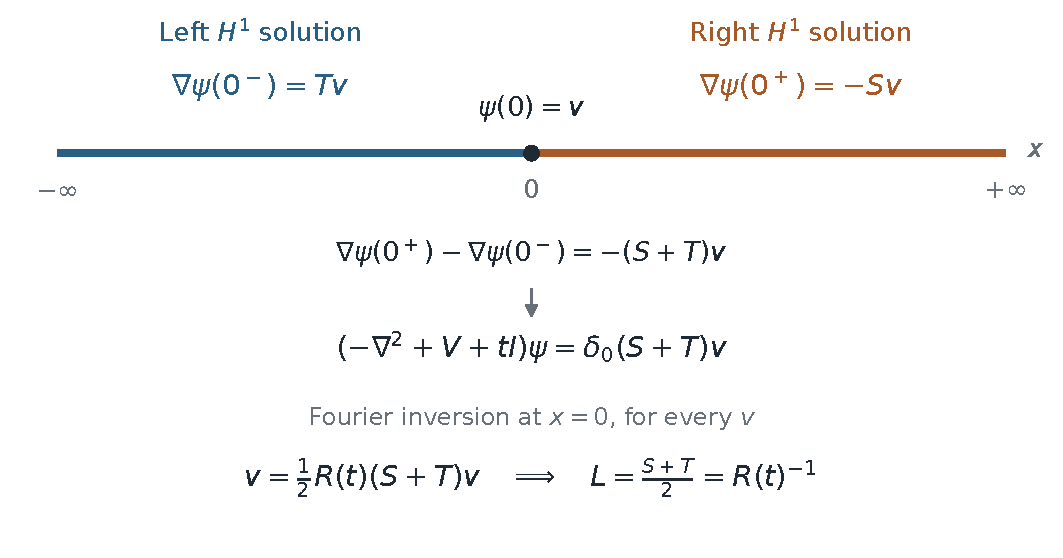
\includegraphics[width=\linewidth]{figures/half-line-gluing.pdf}
 \caption{Gluing the two half-line solutions at a common boundary
 value $v$, for fixed $t>0$ and $\nabla=\partial_x-iB$.
 The colored segments represent the two domains, rather than scalar
 solution profiles.  The jump of the covariant derivative gives the
 point source $\delta_0(S+T)v$.  Fourier inversion at zero, for every
 $v$, identifies the averaged boundary map $(S+T)/2$ with $R(t)^{-1}$.
 The separate Hermitian matrices $S$ and $T$ need not be positive.}
 \label{fig:half-line-gluing}
\end{figure}

Define the Hermitian matrices
\begin{equation}\label{eq:trace-LZ-definition}
 L=\frac{S+T}{2}=R(t)^{-1}>0,
 \qquad Z=\frac{S-T}{2}.
\end{equation}
Adding and subtracting the Riccati identities gives
\begin{equation}\label{eq:trace-LZ-identities}
 V+tI=L^2+Z^2+i[B,Z],\qquad
 LZ+ZL+i[B,L]=0.
\end{equation}
In an eigenbasis of $L$, the second identity has diagonal entries
$2L_{jj}Z_{jj}=0$.  Thus $\tr Z=0$.
Multiplying that identity on both sides by $R=L^{-1}$ gives
$i[R,B]=-(ZR+RZ)$, and cyclicity of the trace yields
\[
 i\tr(R[B,Z])=i\tr([R,B]Z)=-2\tr(RZ^2).
\]
Consequently
\begin{equation}\label{eq:trace-RV}
                 \tr\bigl(R(V+tI)\bigr)=\tr L-\tr(RZ^2).
\end{equation}
The correction $\tr(RZ^2)=\tr(ZRZ)$ is nonnegative.

We have expressed the integrated resolvent through $L$ and identified
a nonnegative correction involving $Z$.  To compare the weighted
integral $N$ with $V$, we next need a scalar quantity whose
$t$-derivative contains $\tr R(t)$.  The logarithm of the determinant
provides that quantity, and the same half-line matrices evaluate it.

\subsection{The logarithmic integral and its weighted identity}

Define
\begin{equation}\label{eq:trace-F-definition}
 F(t)=\frac{\tr V}{\sqrt t}
       -\frac1\pi\int_\R
          \log\frac{\det(X_s+tI)}{\det(Y_s+tI)}\,ds.
\end{equation}
The determinants are positive.  Factoring with
$(Y_s+tI)^{1/2}$ shows that the log ratio is $O(|s|^{-2})$ at
infinity, so its integral converges absolutely.  Its $t$-derivative
is the trace of the difference of the two resolvents.  This has an
integrable bound locally uniform for $t>0$, by the same resolvent
identity used above.  In particular $F$ is continuously
differentiable on $(0,\infty)$.

The first Riccati identity gives the factorization
\begin{equation}\label{eq:trace-factorization}
             X_s+tI=(sI-B+iS)(sI-B-iS).
\end{equation}
Let $u_j+iv_j$, $1\leq j\leq n$, be the eigenvalues of $B+iS$,
with algebraic multiplicity.  Lemma~\ref{lem:trace-half-lines}
gives $v_j>0$.  Since $B-iS=(B+iS)^*$, taking determinants in
\eqref{eq:trace-factorization} gives
\[
 \det(X_s+tI)=\prod_{j=1}^n\bigl((s-u_j)^2+v_j^2\bigr).
\]
The denominator in \eqref{eq:trace-F-definition} has the same form,
with centers the eigenvalues of $B$ and widths all equal to
$\sqrt t$.

These centers can be removed when integrating with symmetric
cutoffs.  Indeed, for $h(s)=\log(s^2+v^2)$, the function $h$ is
even and $h'(s)\to0$ at both ends.  For a fixed translation $a$,
\[
 \frac{d}{da}\int_{-r}^r h(s-a)\,ds=h(r+a)-h(r-a)\longrightarrow0
 \quad(r\to\infty),
\]
uniformly for $a$ in bounded intervals.  Integrating in $a$ shows
that the translation changes the symmetric-cutoff integral by a
quantity tending to zero.  After centering the factors, the scalar
identity
\[
 \int_\R\log\frac{s^2+v^2}{s^2+w^2}\,ds=2\pi(v-w),
 \qquad v,w>0,
\]
follows by differentiation and integration in $v$.
Since $\sum_jv_j=\tr S=\tr L$, we obtain
\begin{equation}\label{eq:trace-F-evaluation}
                  F(t)=\frac{\tr V}{\sqrt t}
                         -2\tr(L-\sqrt t I).
\end{equation}

Introduce a second scalar function
\begin{equation}\label{eq:trace-G-definition}
                 G(t)=\tr\bigl(L-2\sqrt t I+tR(t)\bigr).
\end{equation}
For each eigenvalue $r>0$ of $R(t)$,
$r^{-1}-2\sqrt t+t\,r=(1-\sqrt t\,r)^2/r\geq0$, so $G(t)\geq0$.
Taking traces in \eqref{eq:trace-LZ-identities} and using
\eqref{eq:trace-F-evaluation} also gives
\begin{equation}\label{eq:trace-F-positive}
 F(t)=\frac1{\sqrt t}
        \tr\bigl((L-\sqrt t I)^2+Z^2\bigr)\geq0.
\end{equation}
Equations \eqref{eq:trace-RV} and \eqref{eq:trace-F-evaluation}
now imply the exact identity
\begin{equation}\label{eq:trace-FG-identity}
                   \tr(P(t)V)=F(t)+G(t)+\tr(R(t)Z^2).
\end{equation}

This identity supplies all bounds needed at the improper endpoints.
In fact $0\leq F(t),G(t)\leq\tr(P(t)V)$, even though neither
$V$ nor $P(t)$ is assumed positive.  By
\eqref{eq:trace-P-bounds}, both $F$ and $G$ are $O(t^{-1/2})$
at zero and $O(t^{-3/2})$ at infinity.  They are therefore
integrable against $t^\beta\,dt$, and
\begin{equation}\label{eq:trace-F-boundary}
 \lim_{t\downarrow0}t^{\beta+1}F(t)
   =\lim_{t\to\infty}t^{\beta+1}F(t)=0.
\end{equation}
The same identity proves weighted integrability of $\tr(RZ^2)$.

Differentiating \eqref{eq:trace-F-definition} gives
\[
 F'(t)=-\frac{\tr V}{2t^{3/2}}
          -\tr\bigl(R(t)-t^{-1/2}I\bigr).
\]
Substitution from \eqref{eq:trace-F-evaluation} and
\eqref{eq:trace-G-definition} yields
$tF'(t)=-F(t)/2-G(t)$.  Integrate the derivative of
$t^{\beta+1}F(t)$ on a compact subinterval of $(0,\infty)$,
then use \eqref{eq:trace-F-boundary} to pass to the endpoints.
Since $\beta+\tfrac12=\sigma$, the result is
\begin{equation}\label{eq:trace-weighted-balance}
 \int_0^\infty t^\beta G(t)\,dt
       =\sigma\int_0^\infty t^\beta F(t)\,dt.
\end{equation}
In particular, integrating \eqref{eq:trace-FG-identity} gives
\begin{equation}\label{eq:trace-weighted-identity}
 \tr(NV)
   =q c_\sigma\int_0^\infty t^\beta G(t)\,dt
      +c_\sigma\int_0^\infty t^\beta\tr(R(t)Z^2)\,dt.
\end{equation}

The half-line calculation has thus reduced the theorem to a bound
on the weighted integral of $G$.  The last step compares $G(t)$
with a scalar square-root expression evaluated on an arbitrary
positive semidefinite matrix.  Choosing that matrix in terms of
$N$ will produce the exponent $q$ with no loss in the constant.

\subsection{Completion of the trace comparison}

\begin{proof}[Proof of Theorem~\ref{thm:trace}]
The convergence assertions were proved above.  Let $D\geq0$ be an
$n\times n$ matrix and define
\[
 F_0(t,D)=\frac{\tr D}{\sqrt t}
             -2\tr\bigl((tI+D)^{1/2}-\sqrt t I\bigr).
\]
For a scalar eigenvalue $d\geq0$, its contribution to $F_0$ is
\[
 \frac d{\sqrt t}-2\bigl(\sqrt{t+d}-\sqrt t\bigr)
      =\int_0^d\bigl(t^{-1/2}-(t+y)^{-1/2}\bigr)\,dy.
\]
The integrand is nonnegative.  Tonelli's theorem and
\eqref{eq:trace-scaling}, applied to each eigenvalue of $D$, give
\begin{equation}\label{eq:trace-F0-integral}
 c_\sigma\int_0^\infty t^\beta F_0(t,D)\,dt
                    =\frac1p\tr(D^p).
\end{equation}

For $R=R(t)>0$, the Hilbert--Schmidt square
\begin{align}
 \mathcal D_D(t)
  &:=\bigl\|R^{-1/2}-R^{1/2}(tI+D)^{1/2}\bigr\|_{\HS}^2
       \notag\\
  &=\tr\bigl(R^{-1}+R(tI+D)-2(tI+D)^{1/2}\bigr)\geq0
       \label{eq:trace-square}
\end{align}
is valid without a commutation assumption.  Indeed the cross
term is $\tr(tI+D)^{1/2}$ because the adjacent factors
$R^{-1/2}R^{1/2}$ cancel, while cyclicity puts the remaining
quadratic term in the form $\tr(R(tI+D))$.
Using the definitions of $P,G,F_0$, the same square reads
\[
             \mathcal D_D(t)=G(t)-\tr(P(t)D)+F_0(t,D).
\]
All three terms on the right are integrable against $t^\beta\,dt$,
by \eqref{eq:trace-P-bounds}, \eqref{eq:trace-FG-identity}, and
\eqref{eq:trace-F0-integral}.  Hence
\begin{equation}\label{eq:trace-duality}
 c_\sigma\int_0^\infty t^\beta G(t)\,dt
  =\tr(ND)-\frac1p\tr(D^p)
      +c_\sigma\int_0^\infty t^\beta\mathcal D_D(t)\,dt.
\end{equation}

Now assume $N\geq0$ and choose $D=N^{1/\sigma}$.
Since $p=1+\sigma$ and $q=p/\sigma$, we have
\[
           \tr(ND)-\frac1p\tr(D^p)=\frac1q\tr(N^q).
\]
Combining \eqref{eq:trace-duality} with
\eqref{eq:trace-weighted-identity} gives the exact deficit formula
\begin{equation}\label{eq:trace-deficit}
 \tr(NV)-\tr(N^q)
   =c_\sigma\int_0^\infty t^\beta
       \bigl(\tr(R(t)Z(t)^2)
                 +q\,\mathcal D_{N^{1/\sigma}}(t)\bigr)\,dt.
\end{equation}
Both integrands are nonnegative, proving
\eqref{eq:trace-comparison}.
\end{proof}

\begin{remark}\label{rem:trace-commuting}
If $B$ and $V$ commute, condition \eqref{eq:trace-symbol} implies
$V\geq bI$, and simultaneous diagonalization gives
$R(t)=(tI+V)^{-1/2}$ and $N=V^\sigma$.
Then $Z=0$ and $\mathcal D_{N^{1/\sigma}}=0$, so
\eqref{eq:trace-deficit} vanishes.  In general the two nonnegative
terms in that formula retain the comparison despite the absence
of a common eigenbasis.
\end{remark}
